\setcounter{chapter}{14}

\chapter{Miscellaneous Regression Topics}


{\small \textit{Chapter Preview}. This chapter provides a quick tour
of several regression topics that an analyst is likely to encounter
in different regression contexts. The goal of this chapter is to
introduce these topics, provide definitions and illustrate contexts
in which these topics may be applied.}


\section{Mixed Linear Models}\label{S15:MixedLM}\index{regression model!mixed linear}

Although mixed linear models are an established part of statistical
methodology, their use is not as widespread as regression in
actuarial and financial applications. Thus, the section introduces
this modeling framework, beginning with a widely used special case.
After introducing the modeling framework, this section describes
estimation of regression coefficients and variance components.

We begin with the \emph{one-way random effects} model, with model
equation\index{regression model!one-way random effects}
\begin{equation}\label{E15:OneWayRE}
y_{it} = \mu + \alpha_i + \varepsilon_{it}, ~~~~~ t=1, \ldots, T_i,
~~ i=1,\ldots, n.
\end{equation}
We may use this model to represent repeated observations of subject
or group $i$. The subscript $t$ is used to denote replications that
may be over time or multiple group membership (such as several
employees in a firm). Repeated observations over time was the focus
of Chapter 10.

When there is only one observation per group so that $T_i=1$, the
disturbance term represents the unobservable information about the
dependent variable. With repeated observations, we have an
opportunity to capture unobservable characteristics of the group
through the term $\alpha_i$. Here, $\alpha_i$ is assumed to be a
random variable and is known as a \emph{random effect}. Another
approach, introduced in Section 4.3, represented $\alpha_i$ as a
parameter to be estimated using a categorical explanatory variable.

For this model, $\mu$ represents an overall mean, $\alpha_i$ the
deviation from the mean due to unobserved group characteristics and
$\varepsilon_{it}$ the individual response variation. We assume that
$\{\alpha_i\}$ are i.i.d. with mean zero and variance
$\sigma^2_{\alpha}$. Further assume that $\{\varepsilon_{it}\}$ are
i.i.d. with mean zero and variance $\sigma^2$ and are independent of
$\alpha_i$.

One extension of equation (\ref{E15:OneWayRE}) is the basic random
effects model described in Section 10.5, based on model equation
\marginparjed{Mixed effects models are ones that include random as
well as fixed effects.}
\begin{equation}\label{E15:BasicRE}
y_{it} =\alpha_i + \mathbf{x}_{it}^{\prime} \boldsymbol \beta +
\varepsilon_{it}.
\end{equation}
\noindent In this extension, the overall mean $\mu$ is replaced by
the regression function $\mathbf{x}_{it}^{\prime} \boldsymbol
\beta$. This model includes random effects ($\alpha_i$) as well as
fixed effects ($\mathbf{x}_{it}$). \textit{Mixed effects} models are
ones that include random as well as fixed effects.



Stacking the model equations in an appropriate fashion yields an
expression for the \emph{mixed linear model}
\begin{equation}\label{E15:MixedLinModel}
\mathbf{y} = \mathbf{Z} \boldsymbol \alpha +  \mathbf{X} \boldsymbol
\beta +\boldsymbol \varepsilon .
\end{equation}
Here, $\mathbf{y}$ is a $N \times 1$ vector of dependent variables,
$\boldsymbol \varepsilon $ is a $N \times 1$ vector of errors,
\textbf{Z} and \textbf{X} are $N \times q$ and $N \times k$ known
matrices of explanatory variables, respectively, and $\boldsymbol
\alpha $ and $\boldsymbol \beta$ are $q \times 1$ and $k \times 1$
vectors of unknown parameters. In the mixed linear model, the
$\boldsymbol \beta$ parameters are fixed (non-stochastic) and the
$\boldsymbol \alpha $ parameters are random (stochastic).

For the mean structure, we assume E($\mathbf{y}|\boldsymbol \alpha)
= \mathbf{Z} \boldsymbol \alpha +  \mathbf{X} \boldsymbol \beta$ and
E $\boldsymbol \alpha = \mathbf{0}$, so that $\mathrm{E}~\mathbf{y}
= \mathbf{X} \boldsymbol \beta$. For the covariance structure, we
assume Var($\mathbf{y}|\boldsymbol \alpha) = \mathbf{R}$, Var
($\boldsymbol \alpha)= \mathbf{D}$ and Cov($\boldsymbol
\alpha,\boldsymbol \varepsilon ^{\prime} )= \mathbf{0}$. This yields
Var $\mathbf{y} = \mathbf{Z D Z}^{\prime} + \mathbf{R = V}$. In
longitudinal applications, the matrix $\mathbf{R}$ is used to model
the intra-subject serial correlation.


The mixed linear model is quite general and includes many models as
special cases. For a book-length treatment of mixed linear models,
see Pinheiro and Bates (2000). To illustrate, we return to the basic
random effects model in equation (\ref{E15:BasicRE}). Stacking the
replications from the $i$th group, we may write
\begin{equation*}
\mathbf{y}_i =  \alpha_i \mathbf{1}_i +  \mathbf{X}_i \boldsymbol
\beta +\boldsymbol \varepsilon_i,
\end{equation*}
where $\mathbf{y}_i = (y_{i1} , \ldots, y_{iT_i})^{\prime}$ is the
vector of dependent variables, $\boldsymbol \varepsilon_i = (
\varepsilon_{i1} , \ldots,  \varepsilon_{iT_i})^{\prime}$ is the
corresponding vector of disturbance terms, $\mathbf{X}_i =
(\mathbf{x}_{i1} , \ldots, \mathbf{x}_{iT_i})^{\prime}$ is the $T_i
\times k$ matrix of explanatory variables and $\mathbf{1}_i$ is a
$T_i \times 1$ vectors of ones. Stacking the groups $i=1, \ldots, n$
yields equation (\ref{E15:MixedLinModel}) with $\mathbf{y} =
(\mathbf{y}_1^{\prime} , \ldots, \mathbf{y}_n^{\prime})^{\prime}$,
$\boldsymbol \varepsilon = (\boldsymbol \varepsilon_1 ^{\prime},
\ldots, \boldsymbol \varepsilon_n^{\prime})^{\prime}$, $\boldsymbol
\alpha = ( \alpha _1 , \ldots,  \alpha _n)^{\prime}$,

\begin{equation*}
\mathbf{X}= \left(
  \begin{array}{c}
    \mathbf{X}_1 \\
   \vdots \\
    \mathbf{X}_n \\
  \end{array}
\right) ~~~~\mathrm{and}~~~~ \mathbf{Z}= \left(
  \begin{array}{cccc}
   \mathbf{1}_1 & \mathbf{0} & \cdots & \mathbf{0}\\
    \mathbf{0} & \mathbf{1}_2 & \cdots & \mathbf{0}\\
    \vdots & \vdots & \ddots & \vdots \\
\mathbf{0} &  \mathbf{0}& \cdots & \mathbf{1}_n\\
  \end{array}
\right) .
\end{equation*}

Estimation of the mixed linear model proceeds in two stages. In the
first stage, we estimate the regression coefficients $\boldsymbol
\beta$, assuming knowledge of the variance-covariance matrix
$\mathbf V$. Then, in the second stage, components of the
variance-covariance matrix $\mathbf V$ are estimated.


\subsection{Weighted Least Squares}\index{least squares!weighted}

In Section 5.7.3, we introduced the notion of \emph{weighted} least
squares estimates of the regression coefficients of the form
\begin{equation}\label{E15:WLSCoefficients}
\mathbf{b}_{WLS} = \left(\mathbf{X}^{\prime} \mathbf{W}\mathbf{X}
\right)^{-1}\mathbf{X}^{\prime} \mathbf{W}\mathbf{y} .
\end{equation}
The $n \times n$ matrix $\mathbf{W}$ was chosen to be of the form
$\mathbf{W} = diag(w_i)$ so that the $i$th diagonal element of
$\mathbf{W}$ is a weight $w_i$. As introduced in Section 5.7.3, this
allowed us to fit heteroscedastic regression models.

More generally, we may allow $\mathbf{W}$ to be any (symmetric)
matrix (such that $\mathbf{X}^{\prime} \mathbf{W}\mathbf{X}$ is
invertible). This extension allows us to accommodate other types of
dependencies that appear, for example, in mixed linear models.
Assuming only that E $\mathbf{y} = \mathbf{X} \boldsymbol \beta$ and
Var $\mathbf{y} = \mathbf{V}$, it is easy to establish
\begin{equation}\label{E15:WLSProp1}
\mathrm{E}~\mathbf{b}_{WLS} = \boldsymbol \beta
\end{equation}
and
\begin{equation}\label{E15:WLSProp2}
\mathrm{Var}~\mathbf{b}_{WLS} =  \left(\mathbf{X}^{\prime}
\mathbf{W}\mathbf{X} \right)^{-1}
 \left(\mathbf{X}^{\prime} \mathbf{W}\mathbf{V}\mathbf{W}\mathbf{X}
\right)
 \left(\mathbf{X}^{\prime} \mathbf{W}\mathbf{X}
\right)^{-1} .
\end{equation}
Equation (\ref{E15:WLSProp1}) indicates $\mathbf{b}_{WLS} $ is an
unbiased estimator of $\boldsymbol \beta$. Equation
(\ref{E15:WLSProp2}) is a basic result that is used for statistical
inference, including evaluation of standard errors.

\index{least squares!generalized}

The best choice of the weight matrix is the inverse of the
variance-covariance matrix so that $\mathbf{W}=\mathbf{V}^{-1}$.
This choice results in the \emph{generalized least squares
estimator}, commonly denoted by the acronym $GLS$. The variance is
\begin{equation}\label{E15:GLSProp2}
\mathrm{Var}~\mathbf{b}_{GLS} =
 \left(\mathbf{X}^{\prime} \mathbf{V}^{-1}\mathbf{X}
\right)^{-1} .
\end{equation}
This is best in the sense that it can be shown that
$\mathbf{b}_{GLS} = \left(\mathbf{X}^{\prime}
\mathbf{V}^{-1}\mathbf{X} \right)^{-1}\mathbf{X}^{\prime}
\mathbf{V}^{-1}\mathbf{y}$ has minimum variance among the class of
all unbiased estimators of the parameter vector $\boldsymbol \beta$.
This is property is known as the $Gauss-Markov ~Theorem$, an
extension for general variance-covariance matrices $\mathbf{V}$ of
the property introduced in Section 3.2.3.
\index{theorems!Gauss-Markov}


\subsection{Variance Components
Estimation}\label{S15:VarComp}\index{variance components estimation}

Generalized least squares estimation assumes that $\mathbf{V}$ is
known, at least up to a scalar constant. Of course, it is unlikely
that a general $n \times n$ matrix $\mathbf{V}$  could be estimated
from $n$ observations. However, estimation of special cases of
$\mathbf{V}$ is possible and done routinely. Let $\boldsymbol \tau$
denote the vector of parameters that index $\mathbf{V}$; once
$\boldsymbol \tau$ is known, the matrix $\mathbf{V}$  is fully
specified. We call elements of $\boldsymbol \tau$ the \emph{variance
components}. For example, in our basic regression case we have
$\mathbf{V} = \sigma^2 \mathbf{I}$, so that $\boldsymbol \tau =
\sigma^2$. As another example, in the basic one-way random effects
model, the variance structure is described by the variance
components $\boldsymbol \tau = (\sigma^2,
\sigma^2_{\alpha})^{\prime}$.

There are several methods for estimating variance components, some
of which are likelihood based and others that use method of moments.
These methods are readily available in statistical software. To give
readers a feel for the computations involved, we briefly sketch the
procedure based on maximum likelihood using normal distributions.

For normally distributed observations $\mathbf{y}$ with mean E
$\mathbf{y} = \mathbf{X} \boldsymbol \beta$ and Var $\mathbf{y} =
\mathbf{V} = \mathbf{V (\boldsymbol \tau)}$, the logarithmic
likelihood is given by
\begin{equation}\label{E15:MLMLikelihood}
L(\boldsymbol \beta, \boldsymbol \tau ) = - \frac{1}{2} \left[ N \ln
(2 \pi) + \ln \det (\mathbf{V (\boldsymbol \tau)}) + (\mathbf{y} -
\mathbf{X} \boldsymbol \beta)^{\prime} \mathbf{V (\boldsymbol
\tau)}^{-1} (\mathbf{y} - \mathbf{X} \boldsymbol \beta) \right].
\end{equation}

\marginparjed{The generalized least squares estimator
$\mathbf{b}_{GLS}$ is also the maximum likelihood estimator of
$\boldsymbol \beta$.}

\noindent This log-likelihood is to be maximized in terms of the
parameters $\boldsymbol \beta$ and $\boldsymbol \tau$. In the first
stage, we hold $\boldsymbol \tau$ fixed and maximize equation
(\ref{E15:MLMLikelihood}) over $\boldsymbol \beta$. Pleasant
calculations show that $\mathbf{b}_{GLS}$ is in fact the maximum
likelihood estimator of $\boldsymbol \beta$. Putting this into
equation (\ref{E15:MLMLikelihood}) yields the ``profile'' likelihood
\begin{equation}\label{E15:MLMProfileLikelihood}
L_P(\boldsymbol \tau ) = L(\mathbf{b}_{GLS}, \boldsymbol \tau )
\propto - \frac{1}{2}\left[  \ln \det (\mathbf{V (\boldsymbol
\tau)}) + (\mathbf{y} - \mathbf{X} \mathbf{b}_{GLS})^{\prime}
\mathbf{V (\boldsymbol \tau)}^{-1} (\mathbf{y} - \mathbf{X}
\mathbf{b}_{GLS}) \right] ,
\end{equation}
where we have dropped constants that do not depend on $\boldsymbol
\tau$. (The symbol $\propto$ means ``is proportional to.'')

To implement this two-stage procedure, computer software will
typically use ordinary least squares (OLS) estimates \textbf{b} for
starting values. Then, in the second stage, estimates of
$\boldsymbol \tau$ are determined by iterative methods (numerical
optimization) by finding the values of $\boldsymbol \tau$ that
maximize $L(\mathbf{b},\boldsymbol \tau)$. These estimates are then
used to update the regression coefficient estimates using weighted
least squares. This process is continued until convergence is
achieved.

There are two advantages to this two-stage procedure. First, by
decoupling the regression from the variance component parameters
estimation, we can apply any method that we like to the variance
components and then ``plug-in'' these estimates into the regression
component (estimated) generalized least squares estimation. Second,
we have a closed-form expression for the regression estimates. This
is faster computationally than the iterative methods required by
general optimization routines.

\subsection{Best Linear Unbiased Prediction}\index{best linear
unbiased predictors, $BLUP$}

This section develops \emph{best linear unbiased predictors}
(\emph{BLUPs}) in the context of mixed linear models. We introduce
\textit{BLUPs} as the minimum mean square error predictor of a
random variable, \textit{w}. This development is originally due to
Goldberger (1962), who coined the phrase ``best linear unbiased
predictor.'' The acronym \emph{BLUP} was first used by Henderson
(1973).

The generic goal is to \emph{predict} a random variable \textit{w},
such that $\mathrm{E}~ w = \boldsymbol \lambda ^{\prime} \boldsymbol
\beta$ and $\mathrm{Var}~ w = \sigma^2_w$. Denote the covariance
between $w$ and $\mathbf{y}$ as the $1 \times N$ vector
$\mathrm{Cov}(w,\mathbf{y}) =
\mathrm{E}\{(w-\mathrm{E}w)(\mathbf{y}-\mathrm{E}\mathbf{y})^{\prime}
\}$. The choice of $w$, and thus $\boldsymbol \lambda $ and
$\sigma^2_w$, will depend on the application at hand.

Under these assumptions, it can be shown that the $BLUP$ of $w$ is
\begin{equation}\label{E15:BLUP}
w_{BLUP} = \boldsymbol \lambda ^{\prime} \mathbf{b}_{GLS} +
\mathrm{Cov}(w,\mathbf{y})\mathbf{V}^{-1}(\mathbf{y}-\mathbf{X}
\mathbf{b}_{GLS}).
\end{equation}
The $BLUP$ predictors are optimal, assuming the variance components
implicit in $\mathbf{V}$ and $\mathrm{Cov}(w,\mathbf{y})$ are known.
Applications of \emph{BLUP} typically require that the variance
components be estimated, as described in Section \ref{S15:VarComp}.
\emph{BLUPs} with estimated variance components are known as
\emph{empirical BLUPs}, or \emph{EBLUPs}.

There are three important types of choice for $w$,
\begin{itemize}
\item $w=\varepsilon$, resulting in so-called ``$BLUP$ residuals,''
\item random effects, such as $\boldsymbol \alpha$, and
\item future observations, resulting in optimal forecasts.
\end{itemize}

For the first choice, you will find that $BLUP$ residuals are
regularly coded in statistical software packages that fit linear
mixed models. For the second choice, by letting $w$ be an arbitrary
linear combination of random effects, it can be shown that the
$BLUP$ predictor of $\boldsymbol \alpha$ is
\begin{equation}\label{E15:ABLUP}
\mathbf{a}_{BLUP}  =  \mathbf{D Z}^{\prime} \mathbf{V}^{-1}
(\mathbf{y} - \mathbf{X b}_{GLS}).
\end{equation}
For examples of the third choice, forecasting with linear mixed
models, we refer to Frees (2004, Chapters 4 and 8).

To consider an application of equation (\ref{E15:ABLUP}), consider
the following.

\linejed

\textbf{Special case: One-way Random Effects Model}. Consider the
model based on equation (\ref{E15:OneWayRE}) and suppose that we
wish to estimate the conditional mean of the $i$th group, $w=\mu +
\alpha_i.$ Then, direct calculations (see Frees, 2004, Chapter 4)
based on equation (\ref{E15:ABLUP}) show that the $BLUP$ is
\begin{equation}\label{E15:OneWayBLUP}
\zeta_i \bar{y}_i + (1-\zeta_i ) m_{\alpha,GLS} ,
\end{equation}
with weight $\zeta_i = T_i /(T_i + \sigma^2/\sigma^2_{\alpha}) $ and
$GLS$ estimate of $\mu$, $ m_{\alpha,GLS}  = \sum_i \zeta_i
\bar{y}_i / \sum_i \zeta_i$. In Chapter 18, we will interpret
$\zeta_i$ to be a \emph{credibility factor}.


\linejed

\section{Bayesian Regression}\index{regression model!Bayesian}
\index{regression model!normal linear hierarchical model}

With Bayesian statistical models, one views both the model
parameters and the data as random variables. In this section, we use
a specific type of Bayesian model, the \emph{normal linear
hierarchical model} discussed by, for example, Gelman et al. (2004).
As with the two-stage sampling scheme described in Section 3.3.1,
the hierarchical linear model is one that is specified in stages.
Specifically, we consider the following two-level hierarchy:

\begin{enumerate}
\item Given the parameters $\boldsymbol \alpha$ and $\boldsymbol \beta$, the response model is
$\mathbf{y} = \mathbf{Z}\boldsymbol \alpha + \mathbf{X}\boldsymbol
\beta  + \boldsymbol \varepsilon $. This level is an ordinary
(fixed) linear model that was introduced in Chapters 3 and 4.
Specifically, we assume that the vector of responses $\mathbf{y}$
conditional on $\boldsymbol \alpha$ and $\boldsymbol \beta$ is
normally distributed and that E ($\mathbf{y} | \boldsymbol \alpha,
\boldsymbol \beta ) = \mathbf{Z}\boldsymbol \alpha +
\mathbf{X}\boldsymbol \beta$ and Var ($\mathbf{y} | \boldsymbol
\alpha, \boldsymbol \beta)  = \mathbf{R}$.

\item Assume that $\boldsymbol \alpha$ is distributed normally with mean $\boldsymbol{\mu _{\alpha}}$ and variance
$\mathbf{D}$ and that $\boldsymbol \beta$ is distributed normally
with mean $\boldsymbol{\mu _{\beta}}$   and variance
$\boldsymbol{\Sigma _{\beta}}$ , each independent of the other.

\end{enumerate}

The technical differences between the mixed linear model and the
normal hierarchical linear model are:
\begin{itemize}

\item In the mixed linear model, $\boldsymbol \beta$ is an unknown, fixed parameter
whereas in the normal hierarchical linear model, $\boldsymbol \beta$
is a random vector, and

\item the mixed linear model is distribution-free, whereas distributional
assumptions are made in each stage of the normal hierarchical linear
model.

\end{itemize}

Moreover, there are important differences in interpretation. To
illustrate, suppose that $\boldsymbol \beta= \mathbf{0}$ with
probability one. In the classic non-Bayesian, also known as the
\emph{frequentist}, interpretation, we think of the distribution of
$\{\boldsymbol \alpha\}$ as representing the likelihood of drawing a
realization of $\boldsymbol \alpha _i$. The likelihood
interpretation is most suitable when we have a population of firms
or people and each realization is a draw from that population. In
contrast, in the Bayesian case, one interprets the distribution of
$\{\boldsymbol \alpha\}$ as representing the knowledge that one has
of this parameter. This distribution may be subjective and allows
the analyst a formal mechanism to inject his or her assessments into
the model. In this sense the frequentist interpretation may be
regarded as a special case of the Bayesian framework.

The joint distribution of $(\boldsymbol \alpha^{\prime}, \boldsymbol
\beta^{\prime})^{\prime}$ is known as the \emph{prior} distribution.
To summarize, the joint distribution of $(\boldsymbol
\alpha^{\prime}, \boldsymbol \beta^{\prime},
\mathbf{y}^{\prime})^{\prime}$ is

\begin{equation}\label{E15:JointDistn}
\left(
  \begin{array}{c}
    \boldsymbol \alpha \\
    \boldsymbol
\beta \\
    \mathbf{y} \\
  \end{array}
\right) \sim N
 \left(
 \left(
  \begin{array}{c}
    \boldsymbol {\mu_{\alpha}} \\
    \boldsymbol
{\mu_{\beta}} \\
    \mathbf{Z}\boldsymbol {\mu_{\alpha}} + \mathbf{X}\boldsymbol {\mu_{\beta}}\\
  \end{array}
\right) ,
 \left(
  \begin{array}{ccc}
    \mathbf{D} & \mathbf{0} & \mathbf{DZ}^{\prime} \\
  \mathbf{0} & \boldsymbol {\Sigma_{\beta}}& \boldsymbol {\Sigma_{\beta}}\mathbf{X}^{\prime} \\
    \mathbf{ZD} &  \mathbf{X}\boldsymbol {\Sigma_{\beta}} & \mathbf{V}
     + \mathbf{X}\boldsymbol {\Sigma_{\beta}} \mathbf{X}^{\prime}\\
  \end{array}
\right) \right) ,
\end{equation}
where $\mathbf{V = R + Z D }\mathbf{Z}^{\prime}$.

\index{distributions!posterior}\index{distributions!prior}


The distribution of parameters given the data is known as the
\emph{posterior distribution}. To calculate this conditional
distribution, we use standard results from multivariate analysis.
Specifically, the posterior distribution of $(\boldsymbol
\alpha^{\prime}, \boldsymbol \beta^{\prime})^{\prime}$ given
$\mathbf{y}$ is normal. It is not hard to verify that the
conditional mean is
\begin{equation}\label{E15:CondlMean}
\mathrm{E}~ \left(
  \begin{array}{c}
    \boldsymbol \alpha \\
    \boldsymbol
\beta \\
  \end{array}
\right) |  \mathbf{y} =
 \left(
  \begin{array}{c}
    \boldsymbol {\mu_{\alpha}} + \mathbf{DZ}^{\prime}
    (\mathbf{V}
     + \mathbf{X}\boldsymbol {\Sigma_{\beta}}
     \mathbf{X}^{\prime})^{-1}
     (\mathbf{y} -\mathbf{Z}\boldsymbol {\mu_{\alpha}} - \mathbf{X}\boldsymbol
     {\mu_{\beta}})    \\
    \boldsymbol
{\mu_{\beta}} + \boldsymbol {\Sigma_{\beta}}\mathbf{X}^{\prime}
  (\mathbf{V}
     + \mathbf{X}\boldsymbol {\Sigma_{\beta}}
     \mathbf{X}^{\prime})^{-1}
     (\mathbf{y} -\mathbf{Z}\boldsymbol {\mu_{\alpha}} - \mathbf{X}\boldsymbol
     {\mu_{\beta}}) \\
       \end{array}
\right) .
\end{equation}

Up to this point, the treatment of parameters $\boldsymbol \alpha$
and $\boldsymbol \beta$ has been symmetric. In some applications,
such as with longitudinal data, one typically has more information
about the global parameters $\boldsymbol \beta$  than
subject-specific parameters $\boldsymbol \alpha$. To see how the
posterior distribution changes depending on the amount of
information available, we consider two extreme cases.

First, consider the case  $\boldsymbol{\Sigma _{\beta}}=
\mathbf{0}$, so that $\boldsymbol \beta=\boldsymbol{\mu _{\beta}}$
with probability one. Intuitively, this means that $\boldsymbol
\beta$ is precisely known, generally from collateral information.
Then, from equation (\ref{E15:CondlMean}), we have

\begin{equation}\label{E15:CondlMean1}
\mathrm{E}~ (
    \boldsymbol \alpha |  \mathbf{y}) =
    \boldsymbol {\mu_{\alpha}} + \mathbf{DZ}^{\prime}
    \mathbf{V}^{-1}
     (\mathbf{y} -\mathbf{Z}\boldsymbol {\mu_{\alpha}} - \mathbf{X}\boldsymbol
     \beta) .
\end{equation}
Assuming that  $\boldsymbol{\mu _{\alpha}}= \mathbf{0}$, the best
linear unbiased estimator of E ($\boldsymbol \alpha | \mathbf{y}$)
is
\begin{equation*}
\mathbf{a}_{BLUP}  =  \mathbf{D Z}^{\prime} \mathbf{V}^{-1}
(\mathbf{y} - \mathbf{X b}_{GLS}).
\end{equation*}
Recall from equation (\ref{E15:ABLUP}) that $\mathbf{a}_{BLUP}$ is
also the best linear unbiased predictor in the frequentist
(non-Bayesian) model framework.


Second, consider the case where  $\boldsymbol{\Sigma _{\beta}}^{-1}=
\mathbf{0}$. In this case, prior information about the parameter
$\boldsymbol \beta$ is vague; this is known as using a
\emph{diffuse} prior. In this case, one can check that

\begin{equation*}
\mathrm{E}~ (\boldsymbol \alpha | \mathbf{y}) \rightarrow
\mathbf{a}_{BLUP},
\end{equation*}
as $\boldsymbol{\Sigma _{\beta}}^{-1}\rightarrow \mathbf{0}$. (See,
for example, Frees, 2004, Section 4.6.)

Thus, it is interesting that in both extreme cases, we arrive at the
statistic $\mathbf{a}_{BLUP}$ as a predictor of $\boldsymbol
\alpha$. This analysis assumes $\mathbf{D}$ and $\mathbf{R}$  are
matrices of fixed parameters. It is also possible to assume
distributions for these parameters; typically, independent Wishart
distributions are used for $\mathbf{D}^{-1}$ and $\mathbf{R}^{-1}$
as these are conjugate priors.  Alternatively, one can estimate
$\mathbf{D}$ and $\mathbf{R}$ using methods described in Section
\ref{S15:MixedLM}. The general strategy of substituting point
estimates for certain parameters in a posterior distribution is
called \emph{empirical Bayes estimation}.

To examine intermediate cases, we look to the following special
case. Generalizations may be found in Luo, Young and Frees (2001).

\linejed

\textbf{Special Case: One-way Random Effects Model.} We return to
the model considered in equation (\ref{E15:BasicRE}) and, for
simplicity, assume balanced data so that $T_i = T$. The goal is to
determine the posterior distributions of the parameters. For
illustrative purposes, we focus on the posterior means. Thus,
re-writing equation (\ref{E15:BasicRE}), the model is
\begin{equation*}
y_{it} = \beta + \alpha_i + \varepsilon_{it},
\end{equation*}
where we use the random   $\beta \sim N(\mu_{\beta},
\sigma^2_{\beta})$ in lieu of the fixed mean $\mu$. The prior
distribution of $\alpha_i$ is independent with $\alpha_i  \sim  N(0,
\sigma^2_{\alpha})$.

Using equation (\ref{E15:CondlMean}), we obtain the posterior mean
of $\beta$,
\begin{equation}
\hat{\beta} = \mathrm{E}~(\beta| \mathbf{y}) = \left(
\frac{1}{\sigma^2_{\beta}}+
\frac{nT}{\sigma^2_{\varepsilon}+T\sigma^2_{\alpha}} \right)^{-1}
\left( \frac{nT}{\sigma^2_{\varepsilon}+T\sigma^2_{\alpha}} \bar{y}
+ \frac{\mu}{\sigma^2_{\beta}} \right) ,
\end{equation}
after some algebra. Thus, $\hat{\beta}$ is a weighted average of the
sample mean, $\bar{y}$, and the prior mean,  $\mu_{\beta}$. It is
easy to see that $\hat{\beta}$ approaches the sample mean  as
$\sigma^2_{\beta} \rightarrow \infty$, that is, as prior information
about $\beta$ becomes ``vague.'' Conversely, $\hat{\beta}$
approaches the prior mean $\mu_{\beta}$ as $\sigma^2_{\beta}
\rightarrow 0$, that is, as information about becomes ``precise.''


Similarly, using equation (\ref{E15:CondlMean}), the posterior mean
of $\alpha_i$ is
\begin{equation*}
\hat{\alpha_i} = \mathrm{E}~(\alpha_i | \mathbf{y}) = \zeta \left[ (
\bar{y}_i - \mu_{\beta} ) - \zeta_{\beta} (\bar(y) \mu_{\beta} )
\right]
\end{equation*}
where we have that
\begin{equation*}
\zeta = \frac{T \sigma^2_{\alpha}}{\sigma^2_{\varepsilon}+T
\sigma^2_{\alpha}}
\end{equation*}
and define
\begin{equation*}
\zeta_{\beta} = \frac{nT \sigma^2_{\beta}}{\sigma^2_{\varepsilon}+T
\sigma^2_{\alpha}+nT \sigma^2_{\beta}} .
\end{equation*}
Note that $\zeta_{\beta}$ measures the precision of knowledge about
$\beta$. Specifically, we see that $\zeta_{\beta}$ approaches one as
$\sigma^2_{\beta} \rightarrow \infty$, and approaches zero as
$\sigma^2_{\beta} \rightarrow 0$.

Combining these two results, we have that
\begin{equation*}
\hat{\alpha_i} +\hat{\beta} = (1-\zeta_{\beta}) \left[ (1-\zeta)
\mu_{\beta} + \zeta \bar{y}_i \right] + \zeta_{\beta} \left[
(1-\zeta)\bar{y} + \zeta\bar{y}_i \right] .
\end{equation*}
Thus, if our knowledge of the distribution of $\beta$ is vague, then
$\zeta_{\beta} =1$ and the predictor reduces to the expression in
equation (\ref{E15:OneWayBLUP}) (for balanced data). Conversely, if
our knowledge of the distribution of $\beta$ is precise, then
$\zeta_{\beta} =0$ and the predictor reduces to the expression given
in Chapter 18. With the Bayesian formulation, we may entertain
situations where knowledge is available although imprecise.

\linejed

To summarize, there are several advantages of the Bayesian approach.
First, one can describe the entire distribution of parameters
conditional on the data. This allows one, for example, to provide
probability statements regarding the likelihood of parameters.
Second, this approach allows analysts to blend information known
from other sources with the data in a coherent manner. In our
development, we assumed that information may be known through the
vector of $\boldsymbol \beta$ parameters, with their reliability
control through the dispersion matrix $\boldsymbol{\Sigma
_{\beta}}$. Values of $\boldsymbol{\Sigma _{\beta}}=\mathbf{0}$
indicate complete faith in values of $\boldsymbol{\mu _{\beta}}$,
whereas values of $\boldsymbol{\Sigma _{\beta}}^{-1}=\mathbf{0}$
indicate complete reliance on the data in lieu of prior knowledge.

Third, the Bayesian approach provides for a unified approach for
estimating $(\boldsymbol \alpha, \boldsymbol \beta)$. Section
\ref{S15:MixedLM} on non-Bayesian methods required a separate
subsection on variance components estimation. In contrast, in
Bayesian methods, all parameters can be treated in a similar
fashion. This is convenient for explaining results to consumers of
the data analysis. Fourth, Bayesian analysis is particularly useful
for forecasting future responses.


\section{Density Estimation and Scatterplot Smoothing}\label{S15:Density}\index{density
estimation}\index{plots!scatterplot smoothing}\index{density
estimation!kernel}\index{density estimation!Epanechnikov}


When exploring a variable or relationships between two variables,
one often wishes to get an overall idea of patterns without imposing
strong functional relationships. Typically graphical procedures work
well because we can comprehend potentially nonlinear relationships
more readily visually than with numerical summaries. This section
introduces \emph{(kernel) density estimation} to visualize the
distribution of a variable and \emph{scatterplot smoothing} to
visualize the relationship between two variables.

To get a quick impression of the distribution of a variable, a
histogram is easy to compute and interpret. However, as suggested in
Chapter 1, changing the location and size of rectangles that
comprise the histogram can give viewers different impression of the
distribution. To introduce an alternative, suppose that we have a
random sample $y_1, \ldots, y_n$ from a probability density function
f(.). We define the \emph{kernel density estimator}
\begin{equation*}
\hat{\mathrm{f}}(y) = \frac{1}{n b_n} \sum_{i=1}^n
\mathrm{k}\left(\frac{y-y_i}{b_n}\right),
\end{equation*}
where $b_n$ is a small number called a \emph{bandwidth} and k(.) is
a probability density function called a \emph{kernel}.

To develop intuition, we first consider the case where the kernel
k(.) is a probability density function for a uniform distribution on
(-1,1). For the uniform kernel, the kernel density estimate counts
the number of observations $y_i$ that are within $b_n$ units of $y$,
and then expresses the density estimate as the count divided by the
sample size times the rectangle width (that is, the count divided by
$n \times 2 b_n$). In this way, it can be viewed as a ``local''
histogram estimator in the sense that the center of the histogram
depends on the argument $y$.

There are several possibilities for the kernel. Some widely used
choices are:
\begin{itemize}
\item the uniform kernel, $\mathrm{k}(u) = \frac{1}{2}$ for $-1 \leq u
\leq 1$ and 0 otherwise,
\item the ``Epanechikov'' kernel, $\mathrm{k}(u) = \frac{3}{4}(1-u^2)$ for $-1 \leq u
\leq 1$ and 0 otherwise, and

\item the gaussian kernel, $\mathrm{k}(u) = \phi(u)$ for $-\infty <
u < \infty$, the standard normal density function.
\end{itemize}
The Epanechnikov kernel is a smoother version that uses a quadratic
polynomial so that discontinuous rectangles are not used. The
gaussian kernel is yet more continuous in the sense that the domain
is no longer plus or minus $b_n$ but is the whole real line.


\empexjed{WiscNursingHome}\index{datasets!nursing home utilization}

The bandwidth $b_n$ controls the amount of averaging. To see the
effects of different bandwidth choices, we consider a dataset on
nursing home utilization that will be introduced in Section 17.3.2.
Here, we consider occupancy rates, a measure of nursing home
utilization. A value of 100 means full occupancy although because of
the way this measure is constructed, it is possible for values to
exceed 100. Specifically, there are $n=349$ occupancy rates that are
displayed in Figure \ref{F15:KernelDensity1}. Both figures use a
gaussian kernel. The left-hand panel is based on a bandwidth of 0.1.
This panel appears very ragged; the relatively small bandwidth means
that there is little averaging being done. For the outlying points,
each spike represents a single observation. In contrast, the
right-hand panel is based on a bandwidth of 1.374. In comparison to
the left-hand panel, this picture displays a smoother picture,
allowing the analyst to search for patterns and not be distracted by
jagged edges. From this panel, we can readily see that most of the
mass is less than 100 percent. Moreover, the distribution is
left-skewed, with values of 100-120 being rare.

The bandwidth 1.374 was selected using an automatic procedure built
into the software. These automatic procedures choose the bandwidth
to find the best tradeoff between the accuracy and the smoothness of
the estimates. (For this figure, we used the statistical software
``R'' that has Silverman's procedure built in.)\index{density
estimation!Silverman's procedure}


\begin{figure}[htp]
  \begin{center}
    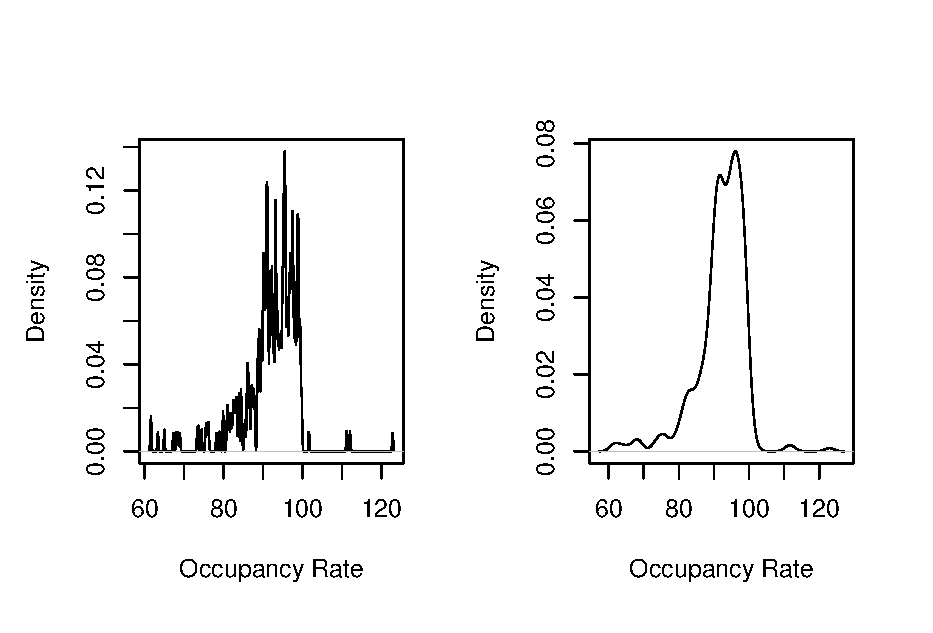
\includegraphics[width=1\textwidth]
        {Chapter15MiscTopics/F15KernelDensity1.eps}
      \end{center}
        \caption {\label{F15:KernelDensity1}
           {\small Kernel Density Estimates of Nursing Home Occupancy Rates With Different Bandwidths.
           The left-hand panel is based on a bandwidth = 0.1, the right-hand panel is based a bandwidth = 1.374.}}
\end{figure}


Kernel density estimates also depend on the choice of the kernel
although this is typically much less important in applications than
the choice of the bandwidth. To show the effects of different
kernels, we show only the $n=3$ occupancy rates that exceeded 110 in
Figure \ref{F15:KernelDensity2}. The left-hand panel shows the
stacking of rectangular histograms based on the uniform kernel. The
smoother Epanechnikov and gaussian kernels in the middle and
right-hand panels are visually indistinguishable. Unless you are
working with very small sample sizes, you will usually not need be
concerned about the choice of the kernel. Some analysts prefer the
uniform kernel because of its interpretability, some prefer the
gaussian because of its smoothness and some prefer the Epanechnikov
kernel as a reasonable compromise.



\begin{figure}[htp]
  \begin{center}
    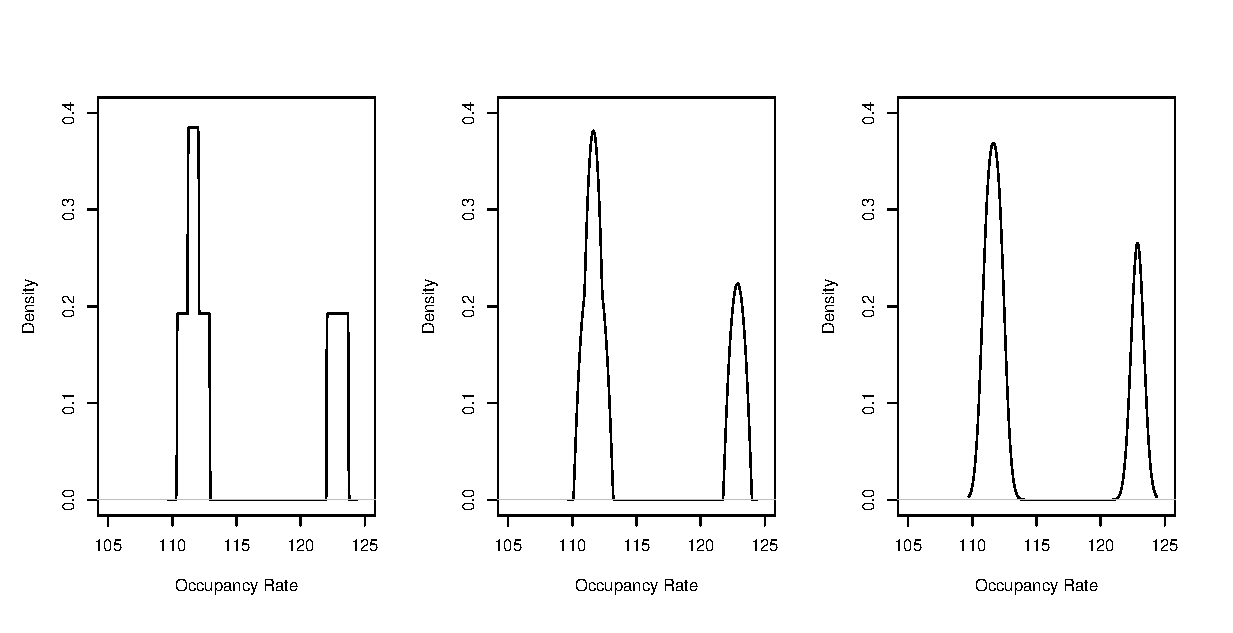
\includegraphics[width=1\textwidth]
        {Chapter15MiscTopics/F15KernelDensity2.eps}
      \end{center}
        \caption {\label{F15:KernelDensity2}
           {\small Kernel Density Estimates of Nursing Home Occupancy Rates With Different Kernels.
           From left to right, the panels use the uniform, Epanechnikov and gaussian kernels.}}
\end{figure}

Some \emph{scatterplot smoothers}, that show relationships between
an $x$ and a $y$, can also be described in terms of kernel
estimation. Specifically, a kernel estimate of the regression
function E ($y |x$) is
\begin{equation*}
\hat{\mathrm{m}}(x) = \frac{\sum_{i=1}^n w_{i,x} y_i}{\sum_{i=1}^n
w_{i,x}}
\end{equation*}
with the ``local'' weight $w_{i,x} = \mathrm{k}\left( (x_i - x)/b_n
\right)$. This is the now-classic Nadaraya-Watson estimator (see,
for example, Ruppert, Wand and Carroll, 2003).

More generally, for a $p$th order local polynomial fit, consider
finding parameter estimates $\beta_0, \ldots, \beta_p$ that minimize
\begin{equation}\label{E15:pthpolynomialfits}
\sum_{i=1}^n \left\{ y_i - \beta_0 - \cdots - \beta_p (x_i - x)^p
\right\}^2 w_{i,x} .
\end{equation} The best value of the intercept $\beta_0$ is taken
to be the estimate of the regression function E ($y |x$). Ruppert,
Wand and Carroll (2003) recommend values of $p$ =1 or 2 for most
applications (the choice $p=0$ yields the Nadaraya-Watson
estimator). As a variation, taking $p=1$ and letting the bandwidth
vary so that the number of points used to estimate the regression
function is fixed results in the \emph{lowess} estimator (for
``local regression'') due to Cleveland (see, for example, Ruppert,
Wand and Carroll, 2003).\index{plots!scatterplot
smoothing!lowess}\index{plots!scatterplot smoothing!Nadaraya-Watson
estimator}

As an example, we used the lowess estimator in Figure 6.11 to get a
sense of the relationship between the residuals and the riskiness of
an industry as measured by INDCOST. As an analyst, you will find
that kernel density estimators and scatterplot smoothers are quite
straightforward to use when searching for patterns and developing
models.

\section{Generalized Additive Models}\label{S15:GAM}\index{regression model!generalized additive, $GAM$}

Classic linear models are based on the regression function
\begin{equation*}
\mu = \mathrm{E} (y| x_1, \ldots, x_k) = \beta_0 + \sum _{j=1}^k
\beta_j x_j .
\end{equation*}
With a generalized linear model (GLM), we have seen that we can
substantially extend applications through a function that links the
mean to the systematic component,
\begin{equation*}
\mathrm{g} \left(\mu  \right) = \beta_0 + \sum _{j=1}^k \beta_j x_j
,
\end{equation*}
from equation (13.1). As in linear models, the systematic component
is linear in the parameters $\beta_j$, not necessarily the
underlying explanatory variables. For example, we have seen that we
can use polynomial functions (such as $x^2$ in Chapter 3),
trigonometric functions (such as $\sin x$ in Chapter 8), binary and
categorizations in Chapter 4 and the ``broken stick'' (piecewise
linear) representation in Section 3.5.2.\index{regression
model!broken stick}


The \emph{generalized additive model} (\emph{GAM}) extends the GLM
by allowing each explanatory variable to be replaced by a function
that may be nonlinear,
\begin{equation}\label{E15:GAMEquation}
\mathrm{g} \left( \mu  \right) = \beta_0 + \sum _{j=1}^k \beta_j
~\mathrm{m}_j(x_j) .
\end{equation}
Here, the function $\mathrm{m}_j(\cdot)$ may differ by explanatory
variable. Depending on the application, $\mathrm{m}_j(\cdot)$ may
include the traditional parametric specifications (such as
polynomials and categorizations) as well as more flexible
nonparametric specifications such as the scatterplot smoothers
introduced in Section \ref{S15:Density}.

For example, suppose that we have a large insurance database and
wish to model the probability of a claim. Then, we might use the
model
\begin{equation*}
\ln \left(\frac{\pi}{1-\pi} \right) = \beta_0 + \sum _{j=1}^k
\beta_j x_j + \mathrm{m}(z) .
\end{equation*}
The left-hand side is the usual logit link function used in logistic
regression, with $\pi$ being the probability of a claim. For the
right-hand side, we might consider a host of rating variables, such
as territory, gender and type of vehicle or house (depending on the
coverage), that are included in the linear component $\beta_0 + \sum
_{j=1}^k \beta_j x_j$. The additional variable $z$ is some
continuous variable (such as age) that we wish to allow for the
possibility of nonlinear effects. For the function $\mathrm{m}(z)$,
we could use a $p$th order polynomial fit with discontinuities at
several ages, such as in equation (\ref{E15:pthpolynomialfits}).

\index{regression model!semiparametric}

This is known as a \emph{semiparametric} model, in that the
systematic component consists of parametric ($\beta_0 + \sum
_{j=1}^k \beta_j x_j$) as well as nonparametric ($\mathrm{m}(z)$)
pieces. Although we do not present the details here, modern
statistical software allows the simultaneous estimation of
parameters from both components. For example, the statistical
software SAS implements generalizes additive models in its PROC GAM
procedure as does the software R through the VGAM package.

The specification of the GAM in equation (\ref{E15:GAMEquation}) is
quite general. For a narrower class, the choice of g($\cdot$) as the
identity function yields the \emph{additive model}. Although
general, the nonparametric forms of $\mathrm{m}_j(\cdot)$ make the
model more flexible, yet the additivity allows us to interpret the
model in much the same way as before. Readers interested in further
information about GAMs will find Ruppert, Wand and Carroll (2003)
and Hastie, Tibshirani and Freedman (2001) to be useful resources.

\bigskip
\section{Bootstrapping}\index{bootstrap}

The \emph{bootstrap} is a general tool for assessing the
distribution of a statistic. We first describe the general procedure
and then discuss ways of implementing it in a regression context.

Suppose that we have an i.i.d. sample $\{z_1, \ldots, z_n \}$ from a
population. From these data, we wish to understand the reliability
of a statistic $\mathrm{S}(z_1, \ldots, z_n )$. To calculate a
bootstrap distribution, we compute:

\begin{enumerate}
\item \textit{Bootstrap Sample}. Generate an i.i.d sample of size $n$,
$\{z^{\ast}_{1r}, \ldots, z^{\ast}_{nr} \}$, from $\{z_1, \ldots,
z_n \}$.
\item \textit{Bootstrap Replication}. Calculate the bootstrap replication,
$S^{\ast}_r =\mathrm{S}(z^{\ast}_{1r}, \ldots, z^{\ast}_{nr} )$.
\end{enumerate}
Repeat steps (i) and (ii) $r=1, \ldots, R$ times, where $R$ is a
large number of replications. In the first step, the bootstrap
sample is randomly drawn from the original sample with replacement.
When repeating steps (i) and (ii), the bootstrap samples are
independent of one another, conditional on the original sample
$\{z_1, \ldots, z_n \}$. The resulting \textit{bootstrap
distribution}, $\{S^{\ast}_1, \ldots, S^{\ast}_R\}$, can be used to
assess the distribution of the statistic $S$.

There are three variations of this basic procedure used in
regression.  In the first variation, we treat $z_i = (y_i,
\mathbf{x}_i)$, and use the basic bootstrap procedure. This
variation is known as \emph{resampling pairs}.

\index{bootstrap!sample}\index{bootstrap!replication}\index{bootstrap!resampling
pairs}\index{bootstrap!resampling
residuals}\index{bootstrap!parametric}


In the second variation, we treat the regression residuals as the
``original'' sample and create a bootstrap sample by sampling the
residuals. This variation is known as \emph{resampling residuals}.
Specifically, consider a generic regression model of the form $y_i =
\mathrm{F}(\mathbf{x}_i, \boldsymbol \theta, \varepsilon_i),$ where
$\boldsymbol \theta$ represents a vector of parameters. Suppose that
we estimate this model and compute residuals $e_i, i=1, \ldots, n$.
In Section 13.5, we denoted the residuals as $e_i = \mathrm{R}(y_i;
\mathbf{x}_i,\widehat{\boldsymbol \theta})$ where the function ``R''
was determined by the model form and $\widehat{\boldsymbol \theta}$
represents the estimated vector of parameters. The residuals may be
the raw residuals, Pearson residuals or some other choice.

Using a bootstrap residual $e^{\ast}_{jr}$, we can create a
pseudo-response
\begin{equation*}
y^{\ast}_{jr}= \mathrm{F}(\mathbf{x}_i, \widehat{\boldsymbol
\theta}, e^{\ast}_{jr}).
\end{equation*}
We can then use the set of pseudo-observations
$\{(y^{\ast}_{1r},\mathbf{x}_1), \ldots,
(y^{\ast}_{nr},\mathbf{x}_n)\}$ to calculate the bootstrap
replication $S^{\ast}_r$. As above, the resulting bootstrap
distribution, $\{S^{\ast}_1, \ldots, S^{\ast}_R\}$, can be used to
assess the distribution of the statistic $S$.

Comparing these two options, the strengths of the first variation
are that it employs fewer assumptions and is simpler to interpret.
The limitation is that it uses a \emph{different} set of explanatory
variables $\{ \mathbf{x}^{\ast}_{1r}, \ldots, \mathbf{x}^{\ast}_{nr}
\}$ in the calculation of each bootstrap replication. Some analysts
reason that their inference about the statistic $S$ is conditional
on the observed explanatory variables $\{ \mathbf{x}_1, \ldots,
\mathbf{x}_n \}$ and using a different set attacks a problem that is
not of interest. The second variation addresses this, but at a cost
of slightly less generality. In this variation, there is a stronger
assumption that the analyst has correctly identified the model and
that the disturbance process $\varepsilon_i = \mathrm{R}(y_i;
\mathbf{x}_i,\boldsymbol \theta)$ is i.i.d.

The third variation is known as a \textit{parametric bootstrap}.
Here, we assume that the disturbances, and hence the original
dependent variables, come from a model that is known up to a vector
of parameters. For example, suppose that we wish the accuracy of a
statistic $S$ from a Poisson regression. As described in Chapter 12,
we assume that $y_i \sim Poisson (\mu_i)$, where $\mu_i =
\exp(\mathbf{x}_i^{\prime} \boldsymbol \beta )$. The estimate of the
regression parameters is $\mathbf{b}$ and so the estimated mean is
$\widehat{\mu}_i = \exp(\mathbf{x}_i^{\prime} \mathbf{b} )$. From
this, we can simulate to create a set of pseudo-responses
\begin{equation*}
y^{\ast}_{ir}\sim Poisson (\widehat{\mu}_i), i=1,\ldots, n,
~~~r=1,\ldots, R.
\end{equation*}
These pseudo-responses can be used to form the $r$th bootstrap
sample, \newline $\{(y^{\ast}_{1r},\mathbf{x}_1), \ldots,
(y^{\ast}_{nr},\mathbf{x}_n)\}$, and from this the bootstrap
replication, $S^{\ast}_r$. Thus, the main difference between the
parametric bootstrap and the first two variations is that we
simulate from a distribution (the Poisson, in this case), not from
an empirical sample. The parametric bootstrap is easy to interpret
and explain because the procedure is similar to the usual Monte
Carlo simulation (see for example, Klugman et al., 2008). The
difference is that with the bootstrap, we use the estimated
parameters to calibrate the bootstrap sampling distribution whereas
this distribution is assumed known in Monte Carlo simulation.


There are two commonly used ways to summarize the accuracy of the
statistic $S$ using the bootstrap distribution, $\{S^{\ast}_1,
\ldots, S^{\ast}_R\}$. The first, a model-free approach, involves
using the percentiles of the bootstrap distribution to create a
confidence interval for $S$. For example, we might use the
$2.5^{th}$ and  $97.5^{th}$ percentiles of $\{S^{\ast}_1, \ldots,
S^{\ast}_R\}$ for a 95\% confidence interval for $S$. For the
second, one assumes some distribution for $S^{\ast}_r,$ typically
approximate normality. With this approach, one can estimate a mean
and standard deviation to get the usual confidence interval for $S$.

\linejed\index{bootstrap!loss reserves}

\textbf{Special Case: Bootstrapping Loss Reserves}. England and
Verrall (2002) discuss bootstrapping loss reserves. As we will see
in Chapter 19, by assuming that losses follow an overdisperse
Poisson, predictions for loss reserves can be obtained by a simple
mechanistic procedure known as the \emph{chain-ladder} technique. To
bootstrap an overdisperse Poisson, as we saw in Chapter 12 this is a
variation of a Poisson model, not a true probability distribution
and so parametric bootstrapping is not readily available. Instead,
England and Verrall showed how to use residual resampling, employing
Pearson residuals.\index{regression model!overdisperse
Poisson}\index{chain ladder}

In many instances, computation of the bootstrap replication
$S^{\ast}_r$ of the statistic can be computationally intensive,
requiring specialized software. However, as pointed out by England
and Verrall, the case of loss reserves with an overdisperse Poisson
is straightforward. One essentially uses the chain-ladder technique
to estimate model parameters and calculate Pearson residuals. Then,
one simulates from the residuals, creates pseudo-responses and
bootstrap distributions. Because simulation is widely available, the
entire procedure can be readily mechanized to work with standard
spreadsheet packages, without the need for statistical software. See
Appendix 3 of England and Verrall (2002) for additional details on
the algorithm.



\linejed






\bigskip


\section{Further Reading and References}

The formula in equations (\ref{E15:BLUP}) does not account for the
uncertainty in variance component estimation. Inflation factors that
account for this additional uncertainty have been proposed (Kackar
and Harville, 1984, but they tend to be small, at least for data
sets commonly encountered in practice. McCulloch and Searle (2001)
provide further discussions.

Silverman (1986) is a now-classic introduction to density
estimation.

Ruppert, Wand and Carroll (2003) provide an excellent book-long
introduction to scatterplot smoothing. Moreover, they provide a
complete discussion of spline-based smoothers, an alternative to
local polynomial fitting.

Efron and Tibshirani (1991) is a now-classic introduction to the
bootstrap.



\bigskip

\textbf{References}


\scalefont{0.9}

\begin{multicols}{2}

Efron, Bradley and Robert Tibshirani (1991). \textit{An Introduction
to the Bootstrap.} Chapman and Hall, London.

England, Peter D. and Richard J. Verrall (2002). Stochastic claims
reserving in general insurance. \emph{British Actuarial Journal} 8,
443-544.

Frees, Edward W. (2004). \textit{Longitudinal and Panel Data:
Analysis and Applications in the Social Sciences.} Cambridge
University Press, New York.

Frees, Edward W., Virginia R. Young and Yu Luo (2001). Case studies
using panel data models. \emph{North American Actuarial Journal} 5
(4), 24-42.

Gelman, A., J. B. Carlin, H. S. Stern and D. B. Rubin (2004).
\textit{Bayesian Data Analysis, Second Edition}. Chapman \& Hall,
New York.

Goldberger, Arthur S. (1962).  Best linear unbiased prediction in
the generalized linear regression model. \textit{Journal of the
American Statistical Association} 57, 369-75.

Hastie, Trevor, Robert Tibshirani and Jerome Friedman (2001). The
\emph{Elements of Statistical Learning: Data Mining, Inference and
Prediction.} Springer, New York.

Henderson, C. R. (1973), Sire evaluation and genetic trends, in
\textit{Proceedings of the Animal Breeding and Genetics Symposium in
Honor of Dr. Jay L. Lush}, 10-41. Amer. Soc. Animal Sci.-Amer. Dairy
Sci. Assn. Poultry Sci. Assn., Champaign, Illinois.

Kackar, R. N. and D. Harville (1984). Approximations for standard
errors of estimators of fixed and random effects in mixed linear
models. \textit{Journal of the American Statistical Association} 79,
853-862.

Klugman, Stuart A, Harry H. Panjer and Gordon E. Willmot (2008).
\emph{Loss Models: From Data to Decisions}. John Wiley \& Sons,
Hoboken, New Jersey.

McCulloch, Charles E. and Shayle R. Searle (2001).
\textit{Generalized, Linear and Mixed Models.} John Wiley \& Sons,
New York.

Pinheiro, Jos\'{e} C. and Douglas M. Bates (2000).
\textit{Mixed-Effects Models in S and S-PLUS}. Springer-Verlag, New
York.

Ruppert, David, M.P. Wand and Raymond J. Carroll (2003).
\textit{Semiparametric Regression}. Cambridge University Press,
Cambridge.

Silverman, B. W. (1986). \textit{Density Estimation for Statistics
and Data Analysis.} Chapman and Hall, London.


\end{multicols}


\scalefont{1.1111}
